
En este caso se supone que la aceleración tiene un sesgo constante asociado. Es por tanto que la matriz $A(t)$ y el vector de estados se pueden reescribir como:
		\begin{equation*}
		A(t) = \begin{pmatrix}0&0&1&0&0&0&0&0&0&0\\[0.3em]0&0&0&1&0&0&0&0&0&0\\[0.3em]0&0&0&0&a^b_x - b_x&a^b_y - b_y&0&0&0&0\\[0.3em]0&0&0&0&0&0&a^b_x -b_x&a^b_y - b_y&0&0\\[0.3em]0&0&0&0&0&\omega^b&0&0&0&0\\[0.3em]0&0&0&0&-\omega^b&0&0&0&0&0\\[0.3em]0&0&0&0&0&0&0&\omega^b&0&0\\[0.3em]0&0&0&0&0&0&-\omega^b&0&0&0\\[0.3em]0&0&0&0&0&0&0&0&1&0\\[0.3em] 0&0&0&0&0&0&0&0&0&1\end{pmatrix} \qquad%
			\vect{x}(t) = \begin{bmatrix} {p_x}(t) \\[0.3em] p_y(t) \\[0.3em] {v_x}(t) \\[0.3em] v_y(t) \\[0.3em] c_{11}(t) \\[0.3em] c_{12}(t) \\[0.3em] c_{21}(t) \\[0.3em] c_{22}(t) \\[0.3em] b_x \\[0.3em] b_y \end{bmatrix}
		\end{equation*}

	Se realiza el mismo proceso de discretización que se utilizó en el ejercicio \ref{sec:ej2}, salvo que donde aparecen las aceleraciones aparecen la diferencia de las mismas con sus sesgos. Luego, al realizar el producto $A\vect{x}$ se obtienen funciones con dependecia de producto de estados, siendo ellas alineales dificultando la estimación del filtro de Kalman. Para solucionarlo, se utiliza el algoritmo de Kalman extendido donde se sigue la dinámica que se linealiza entorno a los estados previos. En la implementación del algoritmo, cada ciclo genera la matriz $A_d = \frac{\partial{f_d}}{\partial \vect{x}}\left| _{\vect{x}=\vect{x}_{k-1/k-1}}\right. $ y a partir de la misma se realiza la predicción y/o corrección del filtro de Kalman tradicional.\\
	\indent En la Figura \ref{fig:ej7} se puede ver la estimación de la trayectoria utilizando dicho algoritmo de estimación. Por medio de las Figuras \ref{fig:7covinn} y \ref{fig:7pos} puede verificarse los resultados del filtro. La Figura \ref{fig:7sesgo} muestra la convergencia de los valores del sesgo en los últimos \SI{100}{\s} de la trayectoria.
	\Juan{Podríamos agregar un gráfico de los valores de $P$ de los sesgos para ver si va saltando o si se va achicando gradualmente}


%\graficarPDF{graf_ej7}{Estimación de la trayectoria.}{fig:ej7}

\begin{figure}[H]
\centering
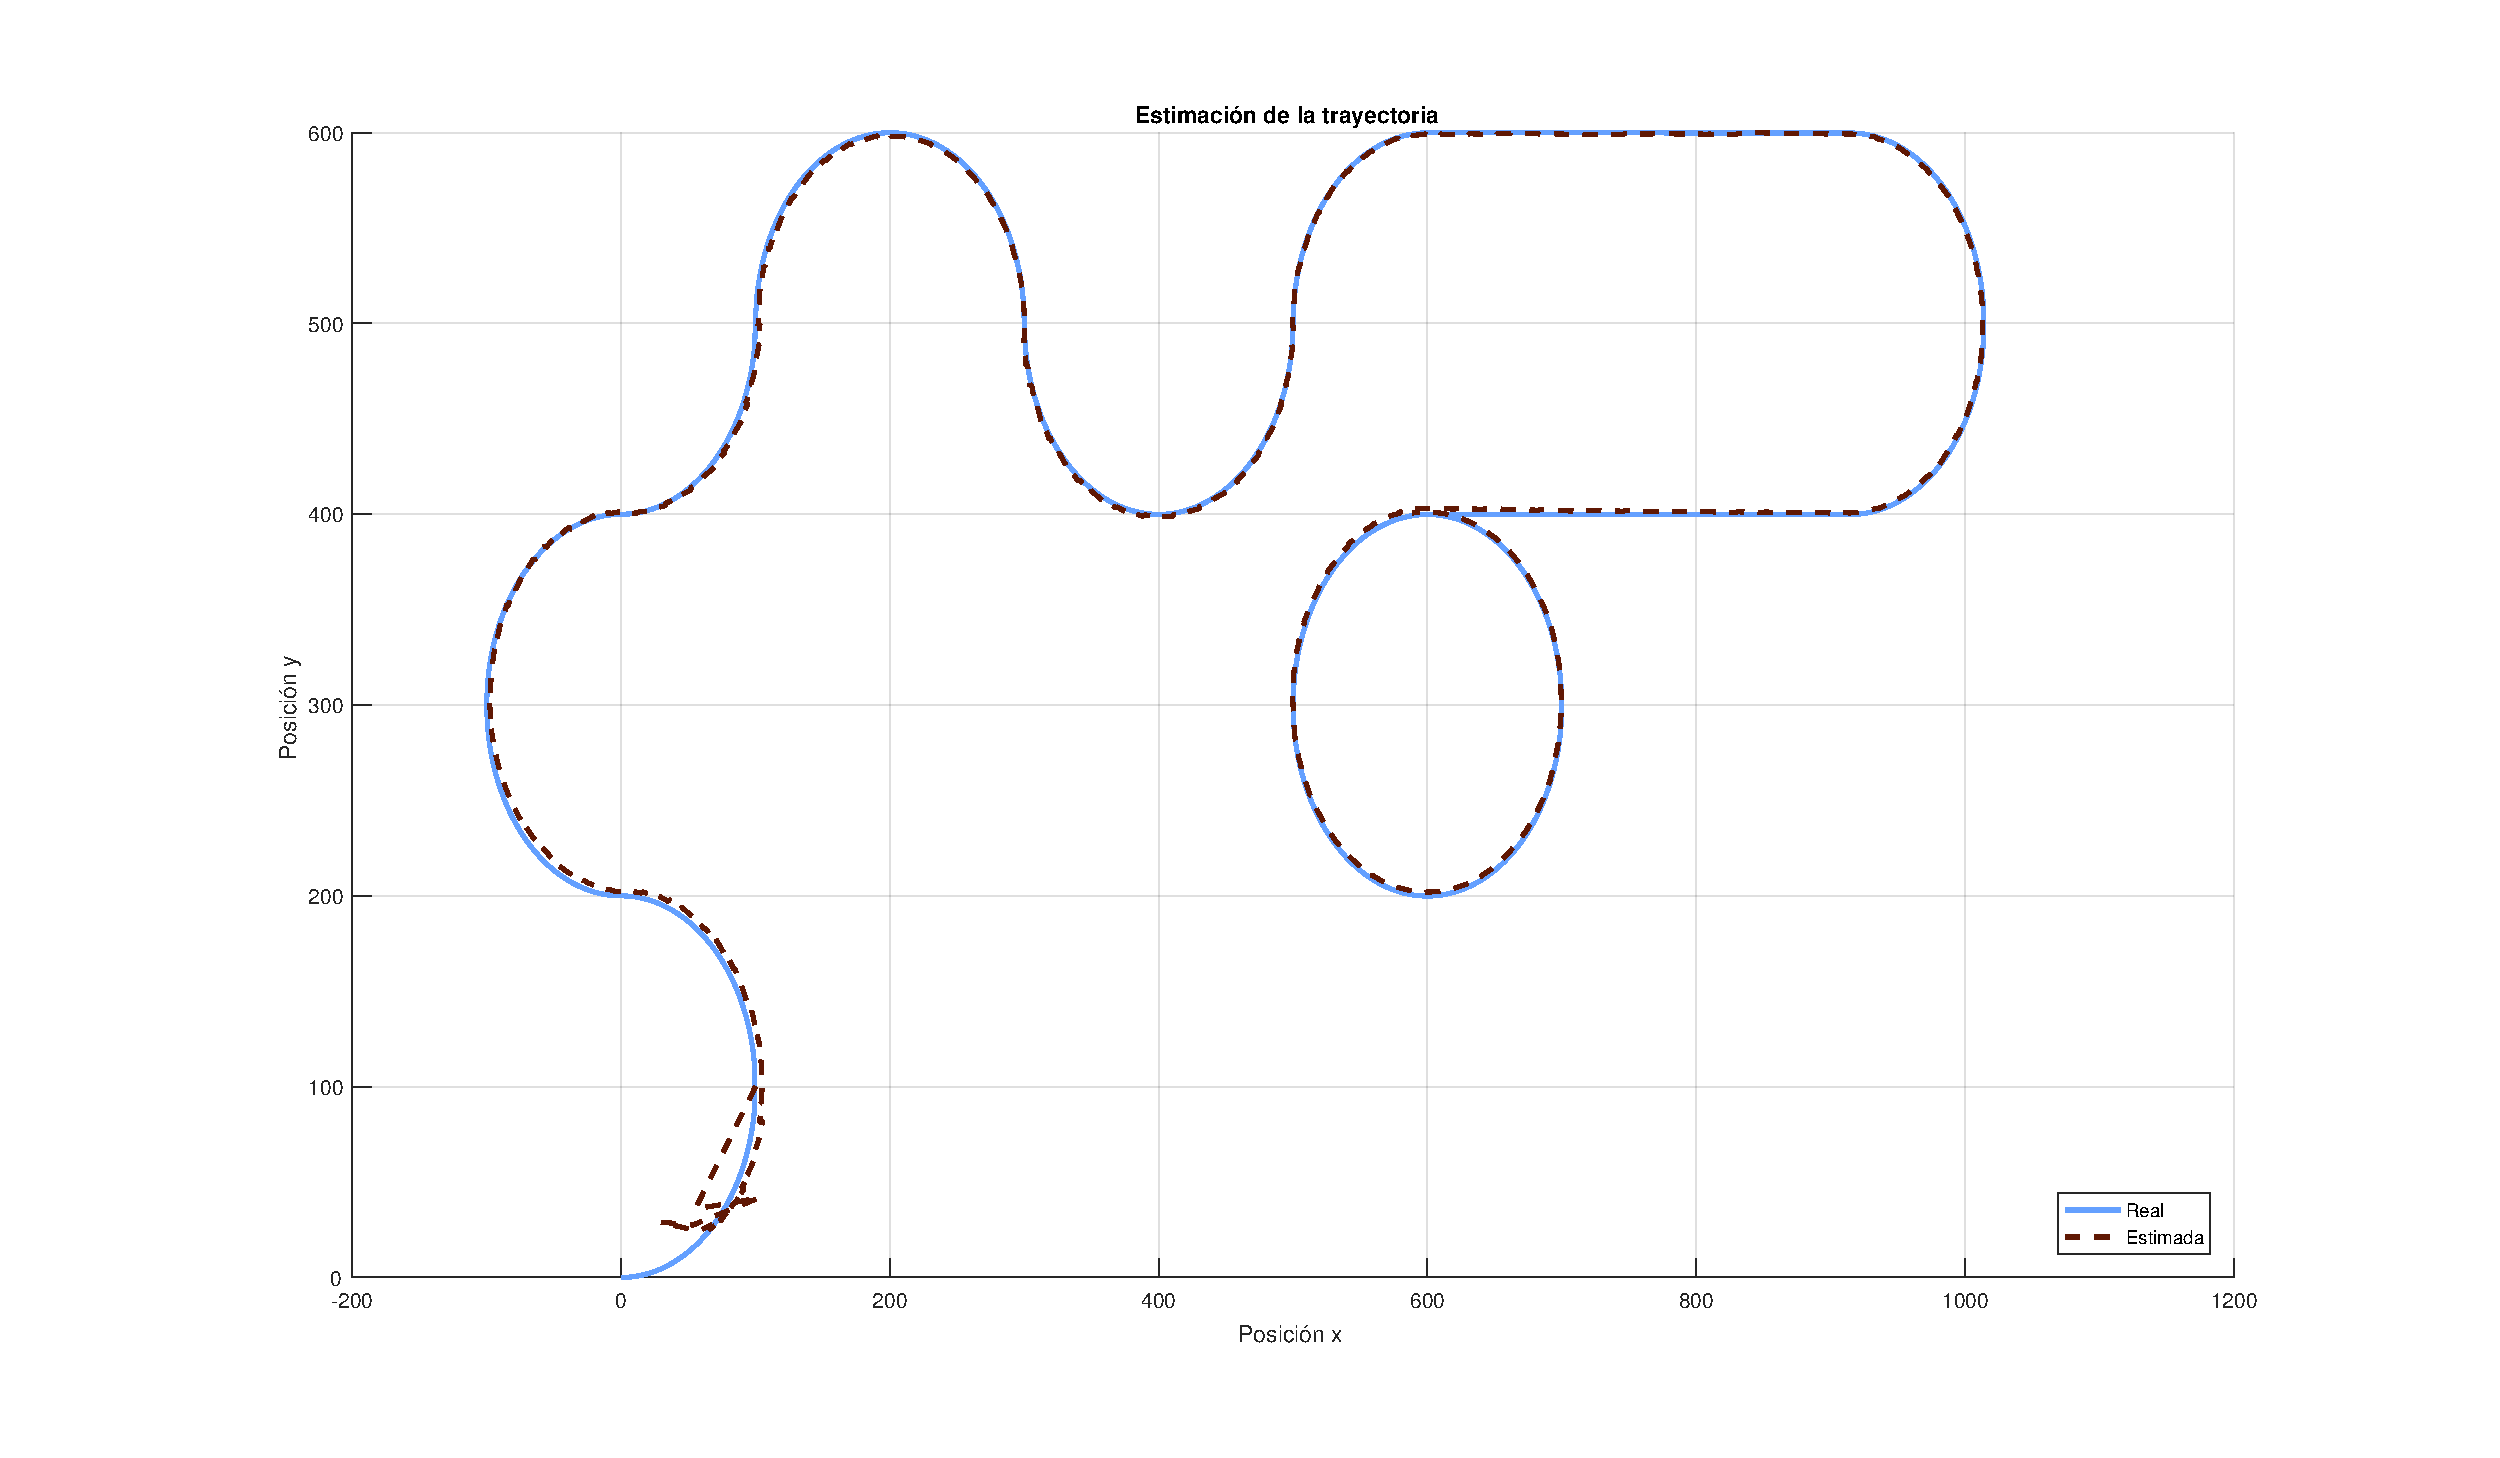
\includegraphics[width=0.85\textwidth, trim= 2cm 2cm 2cm 2cm]{graf_ej7.pdf}
\caption{Estimación de la trayectoria.}
\label{fig:ej7} 
\end{figure}

%\graficarPDF{graf_ej7_covinn}{Innovaciones de las posiciones y velocidades en $x^e$ e $y^e$.}{fig:7covinn}

\begin{figure}[H]
\centering
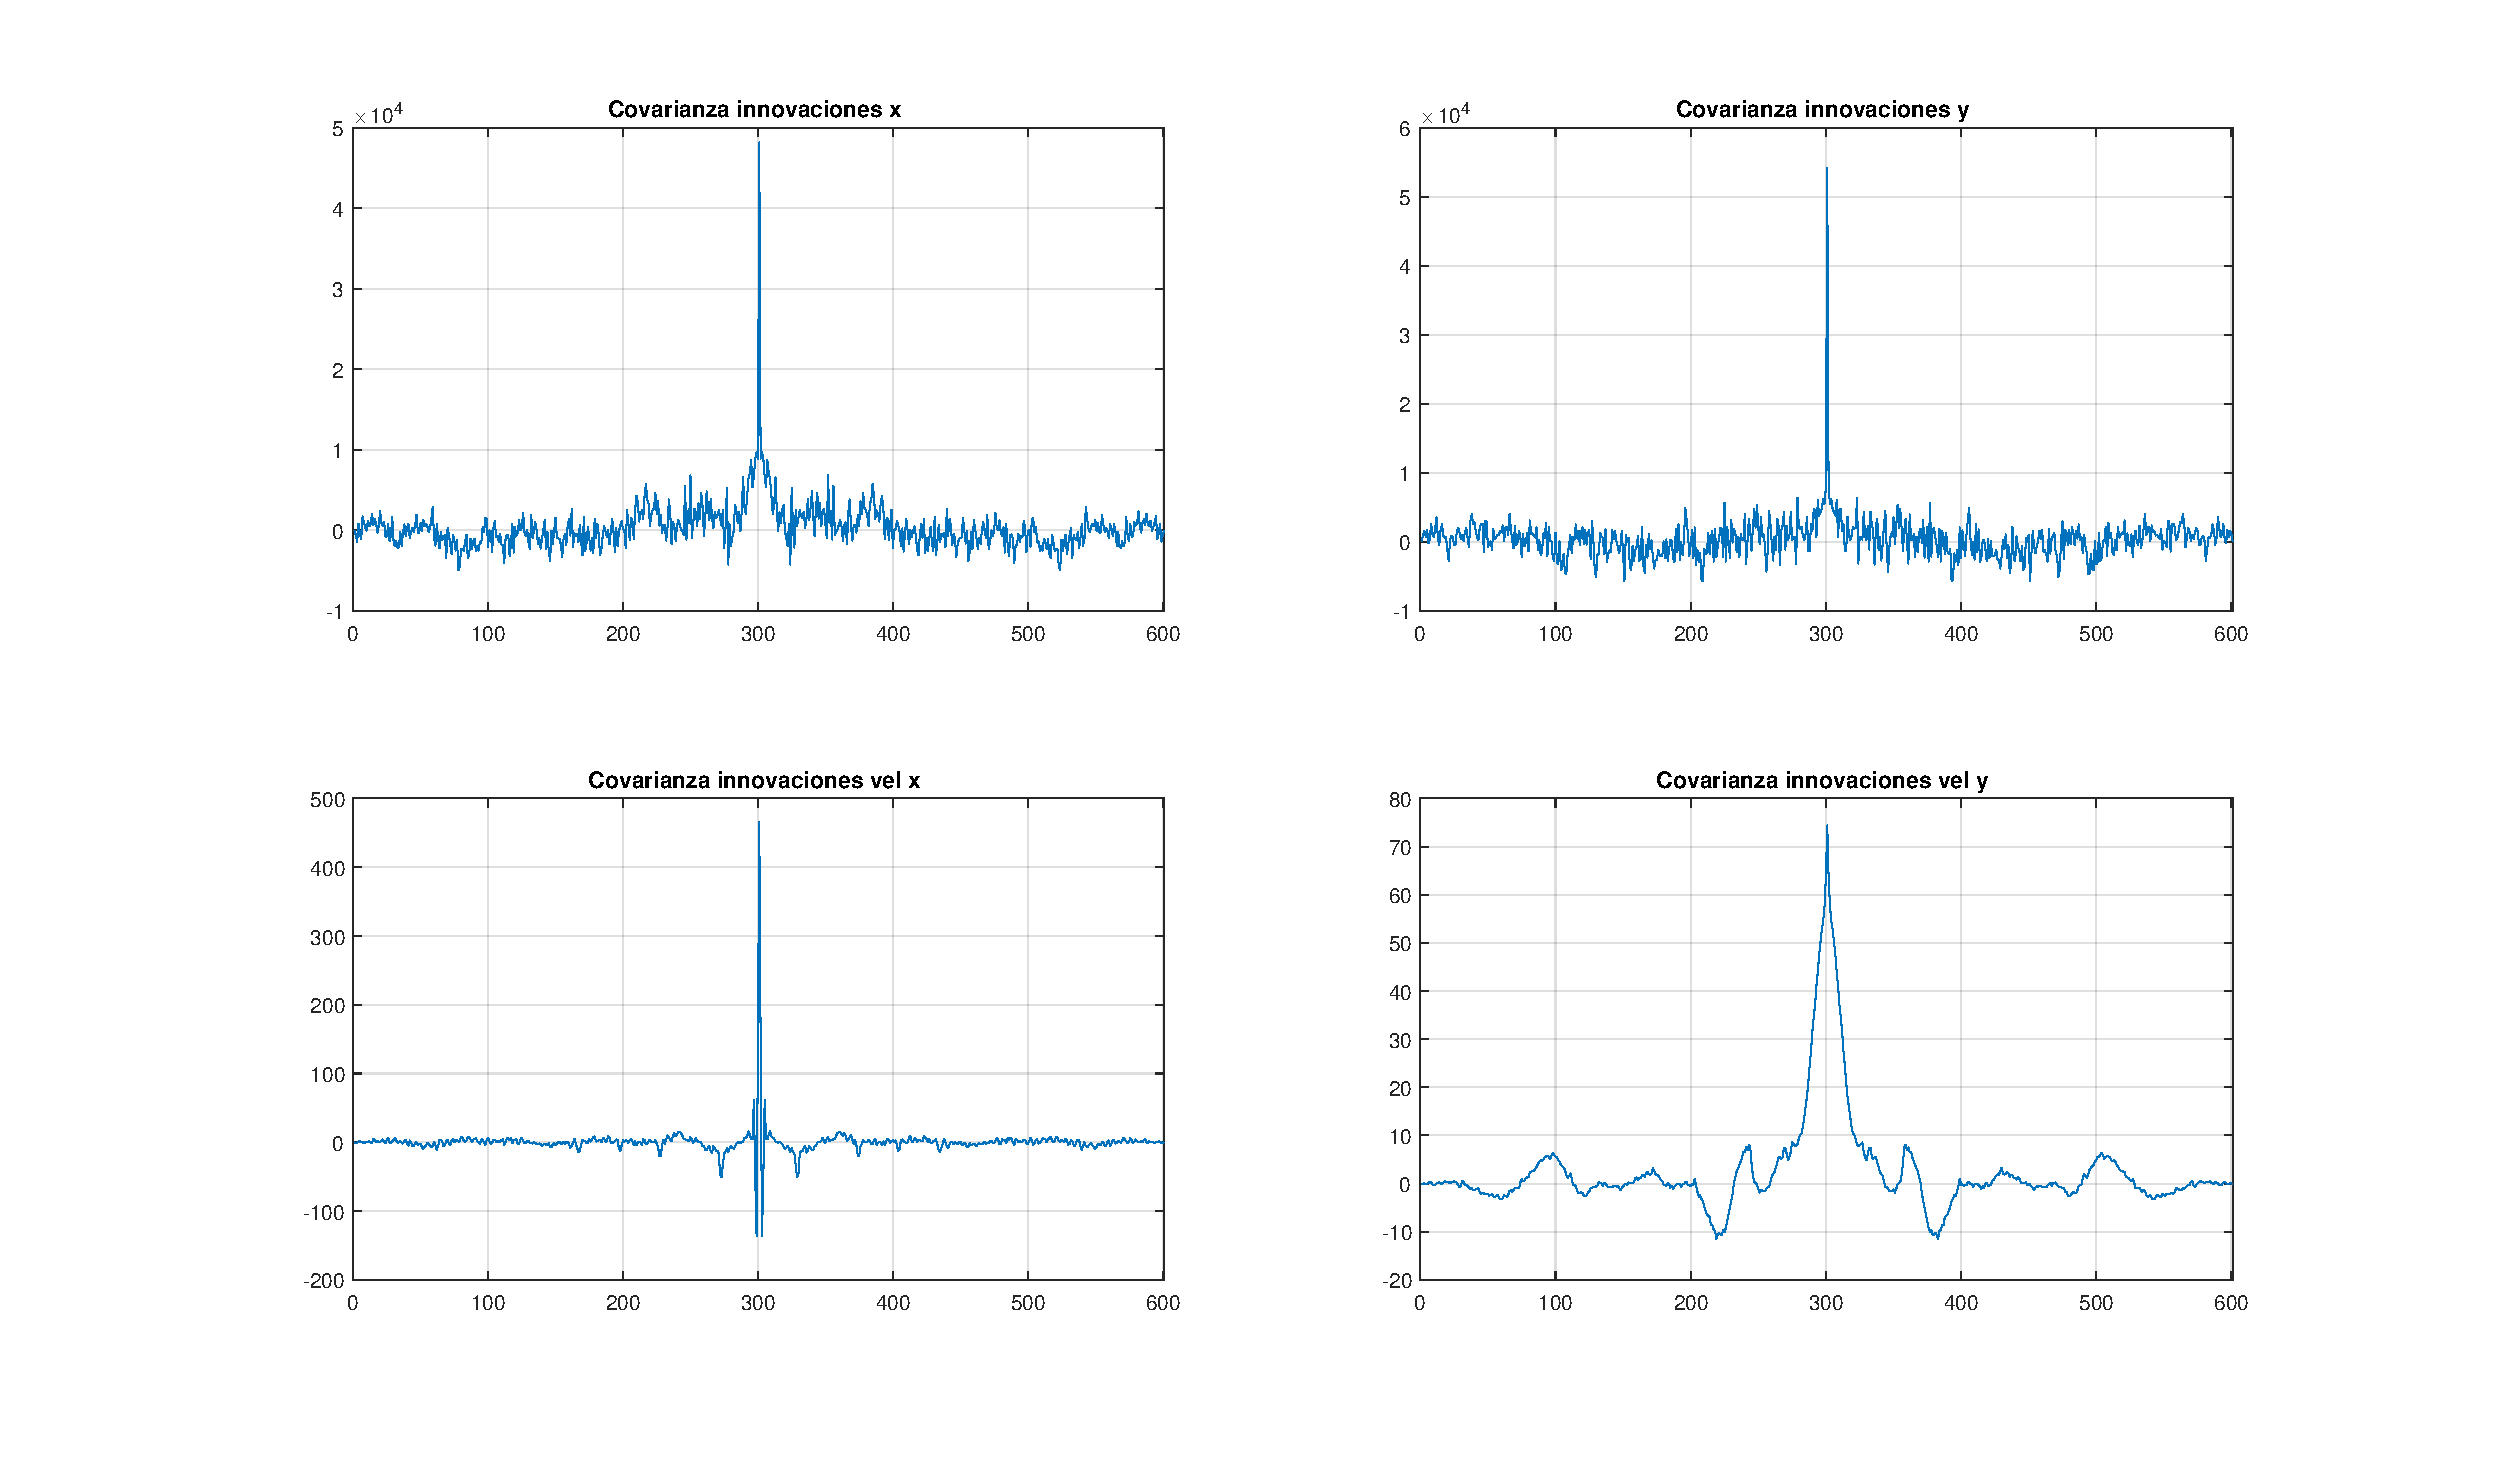
\includegraphics[width=0.85\textwidth,trim= 2cm 2cm 2cm 2cm]{graf_ej7_covinn.pdf}
\caption{Innovaciones de las posiciones y velocidades en $x^e$ e $y^e$.}
\label{fig:7covinn} 
\end{figure}


\pagebreak


%\graficarPDFa{0 10cm 0 10cm}{graf_ej7_pos}{Posición y error de la misma en función del tiempo.}{fig:7pos}

\vspace*{\fill}
\begin{figure}[H]
\centering
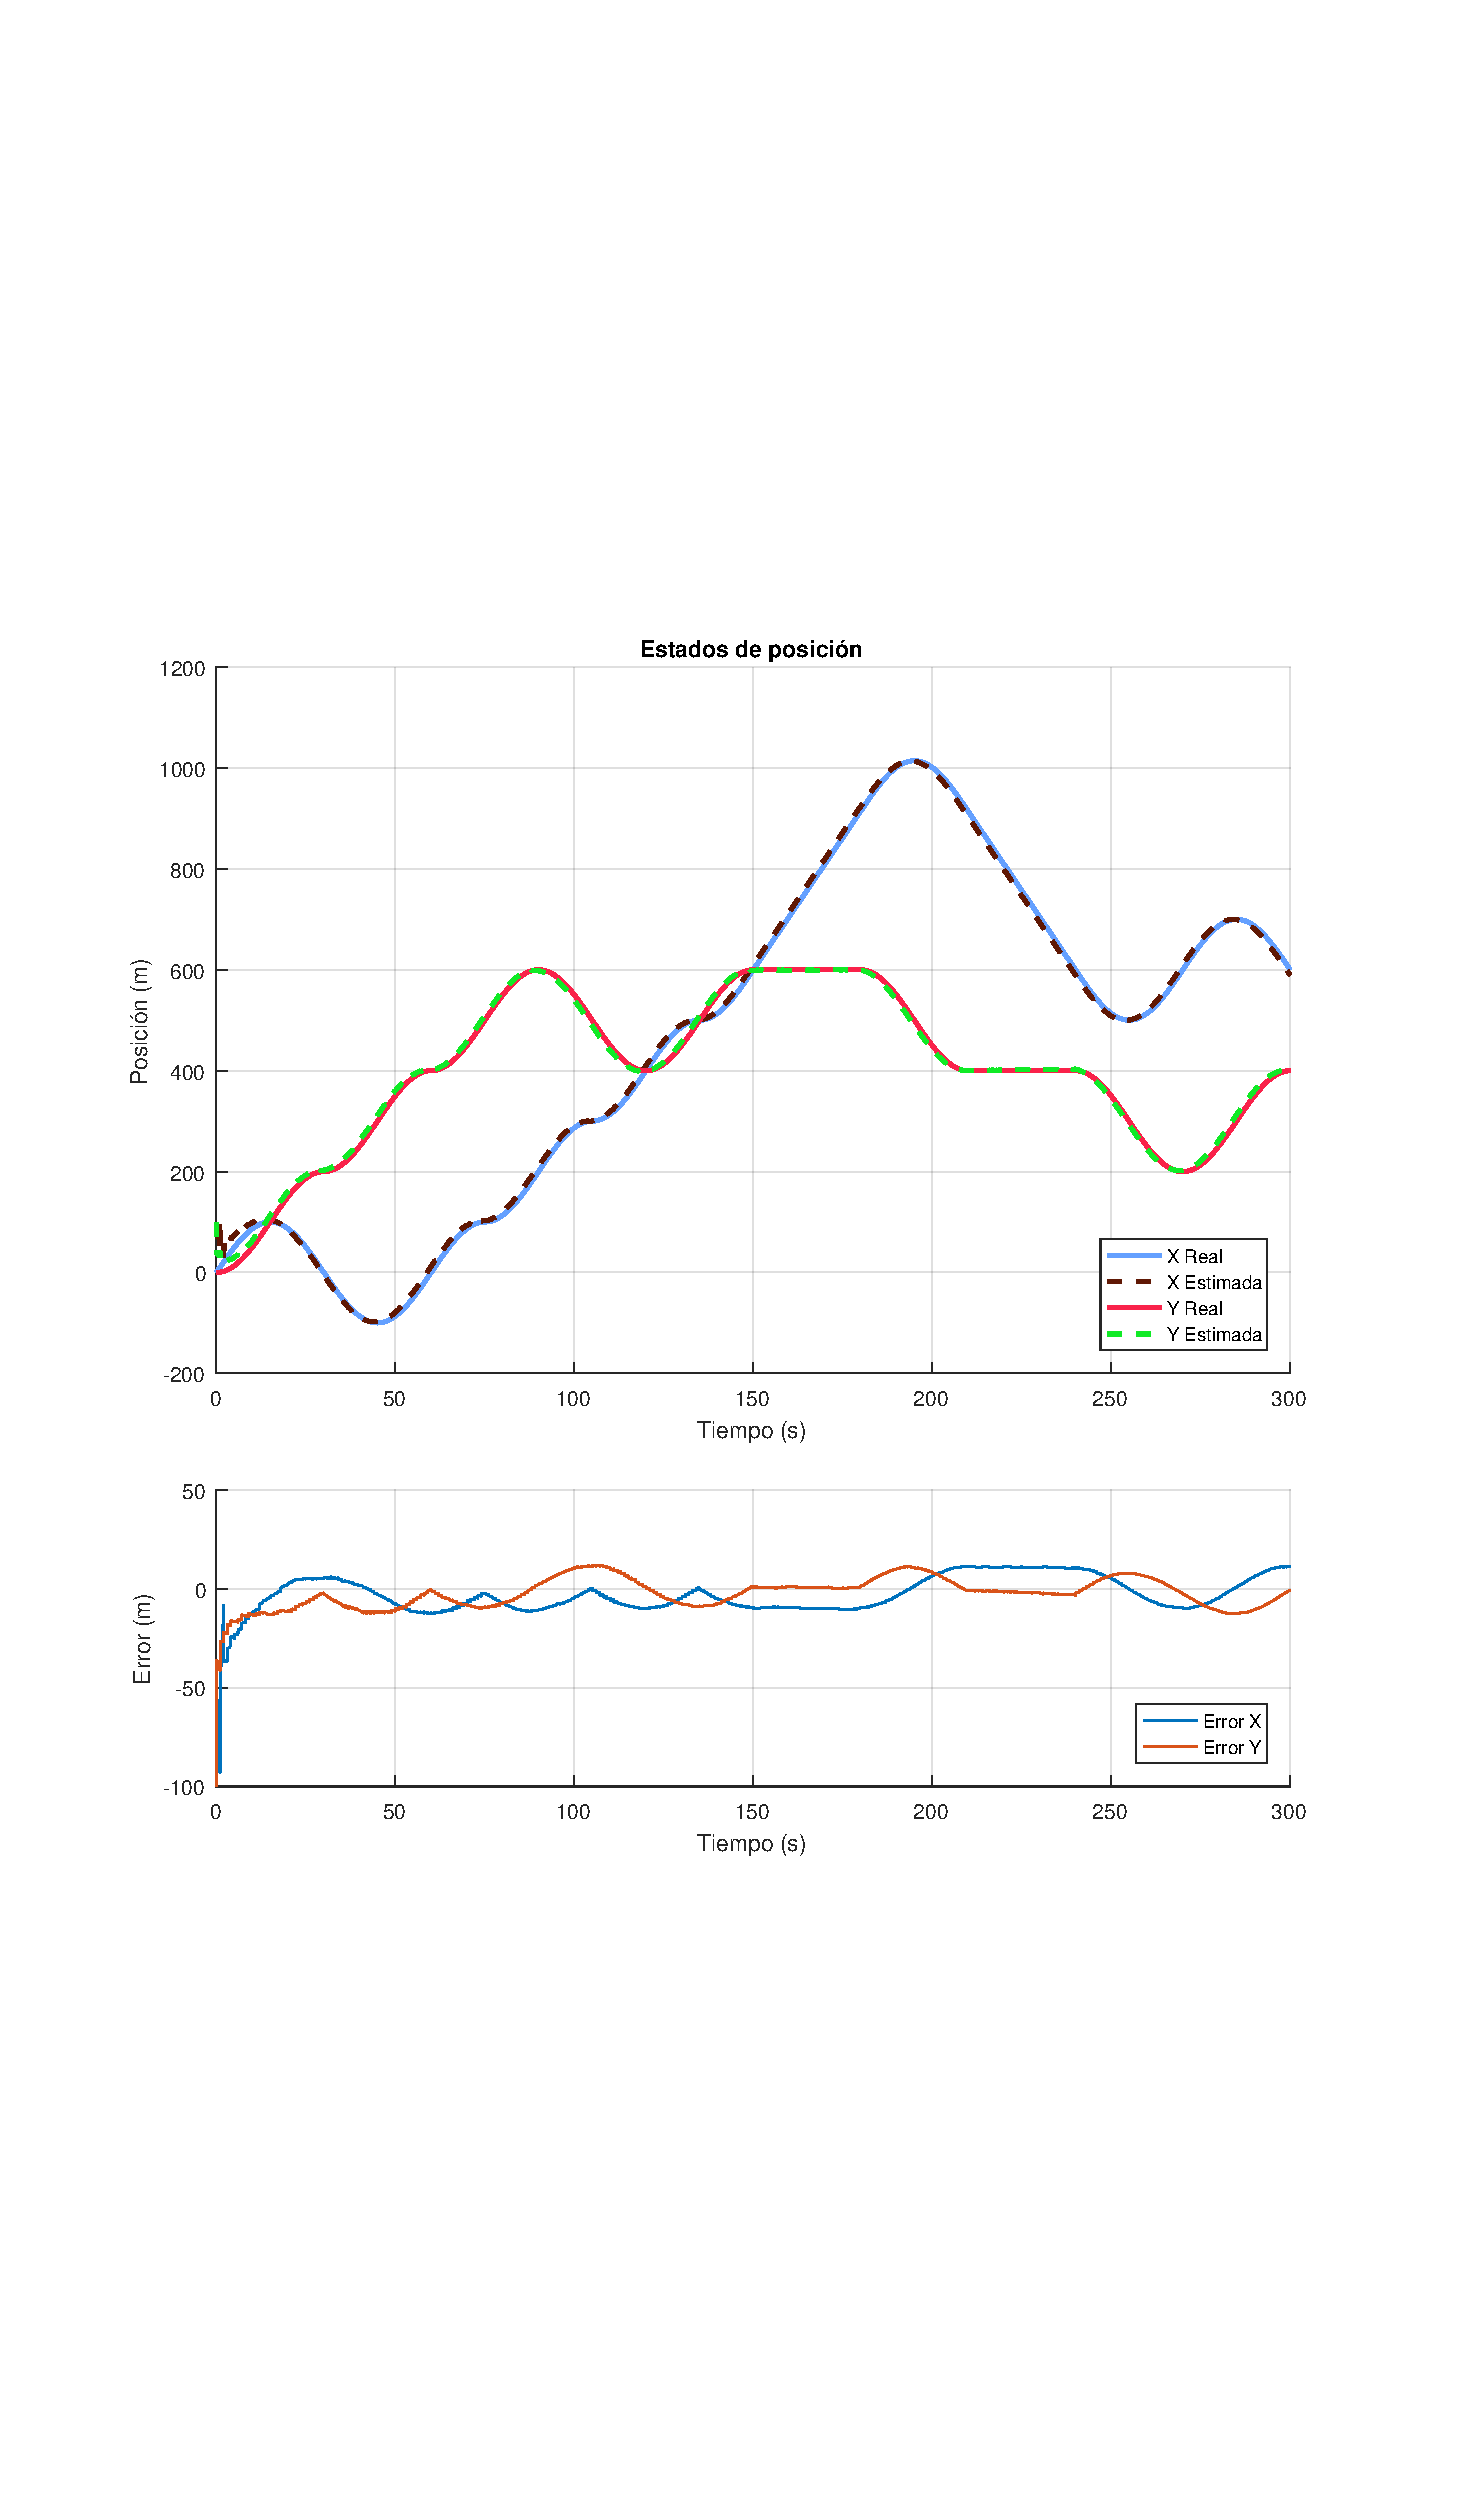
\includegraphics[scale=0.5, trim= 6cm 6cm 6cm 6cm]{graf_ej7_pos.pdf}
\caption{Posición y error en función del tiempo.}
\label{fig:7pos} 
\end{figure}
\vspace*{\fill}

\pagebreak

\graficarPDF{graf_ej7_theta}{Valores de los coeficientes de $C^e_b$ en el tiempo.}{fig:7theta}
\graficarPDF{graf_ej7_vel}{Velocidad real y estimada en función del tiempo.}{fig:7vel}
\graficarPDF{graf_ej7_sesgo}{Valores de los últimos \SI{100}{\s} del sesgo y su convergencia al valor real.}{fig:7sesgo}

%	\begin{equation*}
%		A\, \vect{x} = \begin{bmatrix} 
%			p_x + T\, v_x + (a^b_x - b_x)\frac{T^2}{2}\, c_{11} + (a^b_x - b_x)\frac{T^2}{2} \, c_{12} \\[0.3em]
%			p_y + T\, v_y + (a^b_x - b_x)\frac{T^2}{2}\, c_{21} + (a^b_x - b_x)\frac{T^2}{2} \, c_{22} \\[0.3em]
%			v_x + ac * c11 + ad * c12 \\[0.3em]
%			v_y + ac * c21 + ad * c22 \\[0.3em]
%			s1 * c11 + s2 * c12 \\[0.3em]
%			- s2 * c11 + s1 * c12 \\[0.3em]
%			s1 * c21 + s2 * c22 \\[0.3em]
%			- s2 * c21 + s1 * c22 \\[0.3em]
%			b_x \\[0.3em]
%			b_y \\[0.3em]
%		\end{bmatrix}
%	\end{equation*}



%		\begin{equation*}
%			Ad = \begin{bmatrix} 1& 0& T& 0&                 \frac{T^2(a_x - b_x)}{2}&                 \frac{T^2(a_y - b_y)}{2}&                                 0&                                 0&          -\frac{T^2c11}{2}&          -\frac{T^2c12}{2}\\[0.3em]
%			0& 1& 0& T&                                 0&                                 0&                 \frac{T^2(a_x - b_x)}{2}&                 \frac{T^2(a_y - b_y)}{2}&          -\frac{T^2c21}{2}&          -\frac{T^2c22}{2}\\[0.3em]
%		0& 0& 1& 0& T(a_x - b_x) - \frac{T^2\omega(a_y - b_y)}{2}& T(a_y - b_y) - \frac{T^2\omega(a_x - b_x)}{2}&                                 0&                                 0& \frac{c12\omega T^2}{2} - c11T& \frac{c11\omega T^2}{2} - c12T\\[0.3em]
%		0& 0& 0& 1&                                 0&                                 0& T(a_x - b_x) - \frac{T^2\omega(a_y - b_y)}{2}& T(a_y - b_y) - \frac{T^2\omega(a_x - b_x)}{2}& \frac{c22\omega T^2}{2} - c21T& \frac{c21\omega T^2}{2} - c22T\\[0.3em]
%           0& 0& 0& 0&                   1 - \frac{T^2\omega^2}{2}&                               T\omega&                                 0&                                 0&                     0&                     0\\[0.3em]
%           0& 0& 0& 0&                              -T\omega&                   1 - \frac{T^2\omega^2}{2}&                                 0&                                 0&                     0&                     0\\[0.3em]
%           0& 0& 0& 0&                                 0&                                 0&                   1 - \frac{T^2\omega^2}{2}&                               T\omega&                     0&                     0\\[0.3em]
%           0& 0& 0& 0&                                 0&                                 0&                              -T\omega&                   1 - \frac{T^2\omega^2}{2}&                     0&                     0\\[0.3em]
%           0& 0& 0& 0&                                 0&                                 0&                                 0&                                 0&                     1&                     0\\[0.3em]
%		0& 0& 0& 0&                                 0&                                 0&                                 0&                                 0&                     0&                     1\end{bmatrix}
%		\end{equation*}
